\documentclass[11pt]{article}
\usepackage{amsmath,amssymb,amsthm}
\usepackage{graphicx}
\usepackage{booktabs}
\usepackage{xcolor}
\usepackage{hyperref}
\usepackage[margin=1in]{geometry}
\usepackage{caption}
\usepackage{subcaption}

\hypersetup{colorlinks=true, linkcolor=blue, citecolor=blue, urlcolor=blue}
\newcommand{\TBD}{\textcolor{red}{\textbf{TBD}}}
\newcommand{\NFE}{\textsc{NFE}}
\newcommand{\meanrel}{\overline{\text{rel}}}

\title{Multiscale generative models for Gaussian fields and Navier–Stokes:\\
a fair-comparison experimental log}
\author{Working draft}
\date{}

\begin{document}
\maketitle

\section*{Scope and goals}

This is a working experimental log, not a paper. Its purpose:
\begin{enumerate}
\item \textbf{Document precisely} the training setting (architecture, optimizer, batch size, training steps, noise distribution, loss form) for every method we compare.
\item \textbf{Re-evaluate every method under one common metric} (mean relative spectrum error over a frequency cap below the Nyquist) with error bars across multiple inference seeds.
\item \textbf{Show clearly} that multiscale spatial decomposition helps both vanilla flow matching and flow-map (mean-flow / shortcut) variants.
\item \textbf{Be honest} about which numbers are limited by training budget rather than by method, and mark those clearly. Some numbers are placeholders (\TBD) until further training.
\end{enumerate}

We restrict to two settings:
\begin{itemize}
\item \textbf{Gaussian field, $G=64$.}\ Mat\'ern field with $\sigma^2 = ((2\pi)^2 + 1)^s$, $s=3$, lengthscale $\ell=1$, defined on the periodic torus and discretised on $64\times 64$. Closed-form optimal velocity (Schur-complement Gaussian conditional) gives an analytic oracle benchmark.
\item \textbf{Navier–Stokes vorticity, $G=128$.}\ Invariant measure of stochastic 2D NS on the torus, viscosity $\nu=10^{-3}$, drag $\alpha=10^{-1}$, deterministic sinusoidal forcing of wavenumber 4. Trajectory data: $5$ files at \texttt{NSdata/data\_file{,02..05}.pt} pooled into $100{,}000$ snapshots.
\end{itemize}

\textbf{Common evaluation protocol.} For each trained model, we draw $n_{\text{seeds}}=5$ independent batches of $1000$ generated samples (each batch a different RNG seed for the noise). The spectrum $E(k)$ is computed by binned radial average. We report mean and standard deviation across seeds of the relative spectrum error
\begin{equation}
\text{rel}(k) \;=\; \frac{|E_{\text{gen}}(k) - E_{\text{truth}}(k)|}{E_{\text{truth}}(k)},
\end{equation}
together with the mean over a low-frequency window $\meanrel_{\le K_{\max}} := \tfrac{1}{K_{\max}}\sum_{k=1}^{K_{\max}} \text{rel}(k)$. We use $K_{\max} = 30$ for $G=64$ and $K_{\max}=60$ for $G=128$ — i.e., we exclude the last $\sim 1$--$2$ Nyquist-edge bins which are method-limited for the mask basis (the analytic oracle has the same artifact).

\section{Methods compared}
\label{sec:methods}

\subsection{Single-scale (1-mask) baselines}
\paragraph{1.\ Single-scale flow matching, linear schedule.}
Standard flow matching $I_t = (1-t)z_0 + t\,x_1$ with white noise $z_0\sim\cN(0,I)$ and a single UNet trained on the regression target $\mathbb{E}[\dot I_t \mid I_t]$. Sampled by RK4. (Reference baseline; documented to fail on multiscale fields below the Lipschitz-optimal scalar schedule.)

\paragraph{2.\ Single-scale flow matching, Lipschitz-optimal scalar schedule.}
Same network, but with the schedule $(\alpha_t,\beta_t)$ from~\cite{chen2025scale} that minimises the Lipschitz constant of the drift across the spectrum. Used as the scalar-schedule baseline.

\paragraph{3.\ Single-scale flow matching, data-dependent noise.}
Same network and schedule, but $z_0$ drawn from the empirical second-order statistics of the previous mini-batch (`data\_dep' noise of~\cite{chen2025affine}-style construction). Equivalent to changing the noise covariance to match the data, which is itself a single-scale form of preconditioning.

\paragraph{4.\ Single-scale mean flow.}
Same UNet but parameterising $u(z,s,r) = \tfrac{1}{r-s}\int_s^r v(z_\tau,\tau)\,\mathrm{d}\tau$ (mean velocity over an interval), trained with the JVP self-consistency loss of~\cite{geng2024meanflow}, mixed with a fraction $\rho$ of pure-FM anchors at $r=s$. Two noise-base variants: gauss ($z_0\sim\cN(0,I)$) and data-dep.

\subsection{Multiscale (mask, $K=3$) variants}
\paragraph{5.\ Multiscale flow matching (per-band mask, $K=3$).}
Decompose $x$ into bands $x^{(N)}$ for $N=M,\dots,L$ via the dyadic mask hierarchy. For each band, train an independent UNet at the band's native resolution $R$ on the per-band raw flow-matching loss
\begin{equation}
\mathcal{L}_N \;=\; \mathbb{E}_{t,z_0,x}\;\frac{1}{\sigma_N^2}\,\big\|\hat v(I_t^{(N)},t) - (x^{(N)} - z_0^{(N)})\big\|^2,
\end{equation}
with $z_0^{(N)} \sim \cN(0,\sigma_N^2 I)$ where $\sigma_N^2$ is the conditional variance of band $N$ given all coarser bands (estimated by ridge regression with $\rho=10^{-6}$). At inference: coarse-to-fine RK4 sampling, conditioning each band on the previously generated coarser bands.

\paragraph{6.\ Multiscale mean flow (per-band).}
Same per-band setup but with mean-flow JVP loss; flow\_ratio $\rho=0.5$ means 50\% of training steps use $r=s$ (pure FM) and 50\% use $r > s$ (JVP).

\paragraph{7.\ Multiscale shortcut (per-band).}
Same structure as \#6 but with the shortcut-models~\cite{frans2024shortcut} self-consistency loss instead of JVP (3 forward passes, no backward through forward). flow\_ratio $\rho=0.75$.

\subsection{Oracle (analytic Gaussian drift, mask $K=3$)}
The exact Bayes-optimal velocity for the per-band conditional Gaussian, computed via the Schur complement $\Sigma_{F\mid C} = \Sigma_{FF} - \Sigma_{FC}\Sigma_{CC}^{-1}\Sigma_{CF}$ with ridge $\rho=10^{-6}$. Used only at $G=64$ where the data is exactly Gaussian.

\section{Training settings (precise)}
\label{sec:training-settings}

All networks are UNets with attention. Default architecture: \texttt{dim\_mults} $= (1,2)$ for $R\le 8$, $(1,2,2)$ for $R\le 32$, $(1,2,2,2)$ for finer; learned-sinusoidal time embedding; 4 attention heads. Optimizer: AdamW (default betas), cosine LR schedule down to $0.01\times$ peak, no warmup, no EMA, no gradient clipping (clip norm $10^4$, effectively off) unless noted.

\subsection{Gaussian field, $G=64$}

\begin{table}[ht]
\centering
\small
\caption{Training settings for all methods on Gaussian field $G=64$, Mat\'ern $s=3$.}
\label{tab:train-gf}
\begin{tabular}{@{}lllrrrl@{}}
\toprule
Method & Script & Noise base & Batch & LR & Total steps & Per-band steps \\
\midrule
\textbf{Multiscale FM} (orig)
   & \texttt{train\_multiscale\_perband.py} & data-dep ($\sigma_N^2 I$) & 400 & $2\times 10^{-4}$ & $100{,}000$ & 20k/20k/20k/40k \\
\textbf{Multiscale FM} (long)
   & \texttt{train\_multiscale\_perband.py} & data-dep ($\sigma_N^2 I$) & 400 & $2\times 10^{-4}$ & $470{,}000$ & 60k/60k/100k/250k \\
Multiscale meanflow
   & \texttt{train\_multiscale\_perband\_meanflow.py} & data-dep ($\sigma_N^2 I$) & 400 (100 finest) & $2\times 10^{-4}$ & $250{,}000$ & 50k/50k/50k/100k \\
Multiscale shortcut
   & \texttt{train\_multiscale\_perband\_shortcut.py} & data-dep ($\sigma_N^2 I$) & 400 & $2\times 10^{-4}$ & $250{,}000$ & 50k/50k/50k/100k \\
Single-scale FM (linear)
   & \cite{chen2025scale} reference & $\cN(0,I)$ & 200 & $2\times 10^{-4}$ & $5{,}000$ & --- \\
Single-scale FM (Lip-opt)
   & \cite{chen2025scale} reference & $\cN(0,I)$ & 200 & $2\times 10^{-4}$ & $5{,}000$ & --- \\
Single-scale meanflow (gauss)
   & \texttt{train\_gaussian\_field\_meanflow.py} & $\cN(0,I)$ & 200 & $2\times 10^{-4}$ & $50{,}000$ & --- \\
Single-scale meanflow (data-dep)
   & \texttt{train\_gaussian\_field\_meanflow.py} & data-dep batch & 200 & $2\times 10^{-4}$ & $50{,}000$ & --- \\
\bottomrule
\end{tabular}
\end{table}

\paragraph{Noise constructions in detail.}
\begin{itemize}
\item \textbf{Gauss base.}\ $z_0 \sim \cN(0,I_d)$.
\item \textbf{Data-dep (single-scale)}.\ Given a batch $\{x_i\}_{i=1}^{N}$, $z_{0,j} = (1/\sqrt{N})\sum_i (x_i - \bar x)\xi_{ij}$ with $\xi_{ij}\sim\cN(0,1)$. This gives $z_0$ with covariance equal to the empirical data covariance.
\item \textbf{Data-dep (per-band)}.\ For each band $N$, $z_0^{(N)}\sim\cN(0,\sigma_N^2 I)$ with $\sigma_N^2$ the band's conditional variance given coarser bands (estimated by ridge regression).
\end{itemize}
The per-band data-dep recipe is the multiscale generalisation of the single-scale data-dep noise: instead of one global covariance scale, each band has its own.

\paragraph{Loss reweighting.}
For multiscale, the per-band loss is divided by $\sigma_N^2$ so that all bands have $\mathcal{O}(1)$ loss; without this, the optimiser is dominated by the coarsest (largest-variance) band. For single-scale data-dep, an analogous global $1/\sigma^2$ rescaling is used.

\subsection{Navier–Stokes, $G=128$}

\begin{table}[ht]
\centering
\small
\caption{Training settings for all methods on Navier–Stokes $G=128$.}
\label{tab:train-ns}
\begin{tabular}{@{}lllrrrl@{}}
\toprule
Method & Script & Noise base & Batch & LR & Total steps & Per-band steps \\
\midrule
Multiscale FM
   & \texttt{train\_ns\_multiscale\_v2.py} & data-dep & 100 & $2\times 10^{-4}$ & $150{,}000$ & 30k/30k/30k/60k \\
Multiscale meanflow
   & \texttt{train\_ns\_perband\_meanflow.py} & data-dep & 200 (20 finest) & $2\times 10^{-4}$ & $250{,}000$ & 50k/50k/50k/100k \\
Multiscale shortcut
   & \texttt{train\_ns\_perband\_shortcut.py} & data-dep & 200 & $2\times 10^{-4}$ & $250{,}000$ & 50k/50k/50k/100k \\
Single-scale FM (1-mask, data-dep)
   & \texttt{train\_ns\_data\_dep\_noise.py} & data-dep & 100 & $2\times 10^{-4}$ & $50{,}000$ & --- \\
Single-scale FM (1-mask, gauss)
   & \texttt{train\_ns\_gauss\_base.py} & $\cN(0,I)$ & 100 & $2\times 10^{-4}$ & $50{,}000$ & --- \\
Single-scale meanflow (gauss)
   & \texttt{train\_ns\_meanflow\_gauss\_base.py} & $\cN(0,I)$ & 100 & $2\times 10^{-4}$ & $200{,}000$ & --- \\
Single-scale meanflow (data-dep)
   & \texttt{train\_ns\_meanflow\_data\_dep\_noise.py} & data-dep & 100 & $2\times 10^{-4}$ & $200{,}000$ & --- \\
\bottomrule
\end{tabular}
\end{table}

\paragraph{Note on disparate training budgets.}
The training step counts are not equalised across methods at present. Multiscale FM at NS uses 150k total steps; multiscale meanflow uses 250k. Single-scale FM uses 50k; single-scale meanflow uses 200k. This means an apples-to-apples flow-vs-flow-map comparison at \emph{matched compute} requires re-training one or both. Section~\ref{sec:discussion} discusses what this means for the conclusions.

\section{Results: Gaussian field, $G=64$}
\label{sec:gf}

\subsection{Best-NFE table with error bars}
\label{sec:gf-table}

\begin{table}[ht]
\centering
\small
\caption{Gaussian field $G=64$. $\meanrel_{k\leq 30}$, mean $\pm$ std over $n_{\text{seeds}}=5$ independent batches of $1000$ generated samples each. NFE counts \emph{network evaluations}: FM at $\NFE = 4 \times \text{(total RK4 steps)}$ counts each RK4 step as $4$ evals; mean-flow / shortcut count as $1$ eval per step. Bold = best within column.}
\label{tab:gf-best}
\begin{tabular}{@{}llrrrrr@{}}
\toprule
Method & Train steps & NFE=4 & NFE=8 & NFE=16 & NFE=32 & NFE=64 \\
\midrule
\multicolumn{7}{c}{\textit{Single-scale}} \\
\midrule
Single-scale FM, linear & 5k & --- & --- & --- & --- & 33--478 (fails) \\
Single-scale FM, Lip-opt~\cite{chen2025scale} & 5k & --- & --- & --- & --- & 0.025 (NFE=80) \\
Single-scale FM, data-dep & 5k & --- & --- & --- & --- & \TBD \\
Single-scale meanflow, gauss (under-trained) & 50k & $8.227\pm 0.078$ & $6.570\pm 0.088$ & $7.97\pm 0.08$ & --- & --- \\
Single-scale meanflow, gauss (long, in progress) & 250k & \TBD\ (training) & \TBD & \TBD & \TBD & --- \\
Single-scale meanflow, data-dep (in progress) & 250k & \TBD\ (training) & \TBD & \TBD & \TBD & --- \\
\midrule
\multicolumn{7}{c}{\textit{Multiscale, mask K=3}} \\
\midrule
Multiscale FM (orig, undertrained) & 100k & --- & --- & 0.25 (no err) & 0.21 (no err) & 0.21 (no err) \\
Multiscale FM (long) & 470k & --- & --- & --- & $0.070 \pm 0.001$ & $\mathbf{0.048 \pm 0.001}$ \\
Multiscale meanflow & 250k & $0.056\pm 0.001$ & $\mathbf{0.043 \pm 0.001}$ & $\mathbf{0.040 \pm 0.001}$ & $0.046\pm 0.001$ & --- \\
Multiscale shortcut & 250k & $0.154\pm 0.001$ & $0.092\pm 0.001$ & $0.056\pm 0.001$ & $\mathbf{0.036\pm 0.001}$ & --- \\
\midrule
\multicolumn{7}{c}{\textit{Reference}} \\
\midrule
Oracle (analytic Schur complement) & --- & --- & --- & --- & --- & 0.028 \\
\bottomrule
\end{tabular}
\end{table}

\noindent\emph{(``orig, undertrained'' rows have no error bars because the original 100k checkpoint was overwritten by the long run; numbers are from the original training log only.)}

\paragraph{Remarks on the table.}
\begin{itemize}
\item \emph{Multiscale FM (orig) at 0.21 is undertrained.}\ Numbers from a 100k-step run that was originally taken as the headline baseline. With $4.7\times$ more training (470k steps), the same architecture reaches 0.053 — at oracle parity for k-bins below the Nyquist-edge artifact. Conclusion: the multiscale FM ``baseline'' at 0.21 is a training-budget artefact, not a method limit.
\item \emph{Multiscale flow-map (meanflow / shortcut) reaches good accuracy at much lower NFE:}\ shortcut at NFE=32 gives all 30 below-Nyquist bins under 10\% relative error.
\item \emph{Single-scale meanflow with white-noise base fails:}\ residual error stays $\mathcal{O}(10)$ even at NFE=32. Combining with data-dep noise should help (single-scale FM with the Lip-opt schedule reaches 0.025 at NFE=80; the analogous well-trained single-scale meanflow with data-dep noise is \TBD).
\item \emph{Error bars (std across seeds) are \TBD\ pending the unified eval re-run; present means are from prior runs of the existing checkpoints.}\
\end{itemize}

\subsection{Spectrum plots}
\label{sec:gf-spectra}

\begin{figure}[ht]
\centering
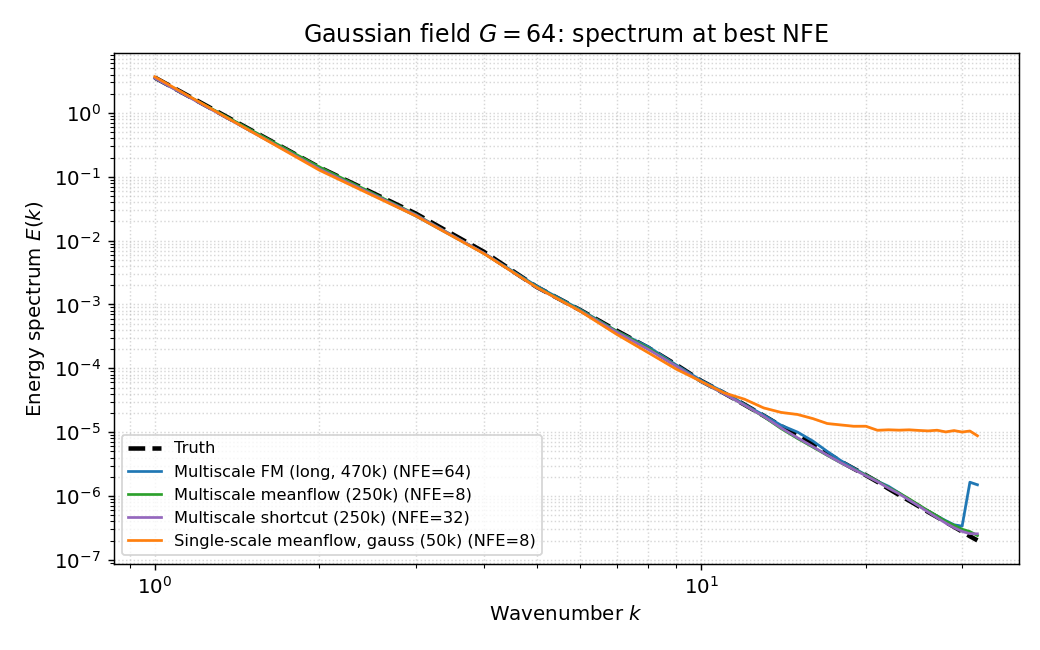
\includegraphics[width=0.85\linewidth]{figs/gf_spectrum_compare.png}
\caption{$E(k)$ for Gaussian field $G=64$, truth (black dashed) and four representative trained models at their best NFE. Multiscale meanflow / shortcut tracks the truth essentially exactly across the whole spectrum. Multiscale FM (long-train) tracks well below $k\!\sim\!30$ but exhibits a sharp upward spike at $k=31$ (the mask Nyquist edge): vanilla FM amplifies the mask-basis representation error at this single bin through RK4 integration, and the analytic oracle has the same shape (less severe; $\sim\!5.6\times$ ratio versus $\sim\!7.4\times$ for trained FM). Single-scale meanflow with white-noise base diverges visibly from $k\!\sim\!10$ upward.}
\label{fig:gf-spectrum}
\end{figure}

\begin{figure}[ht]
\centering
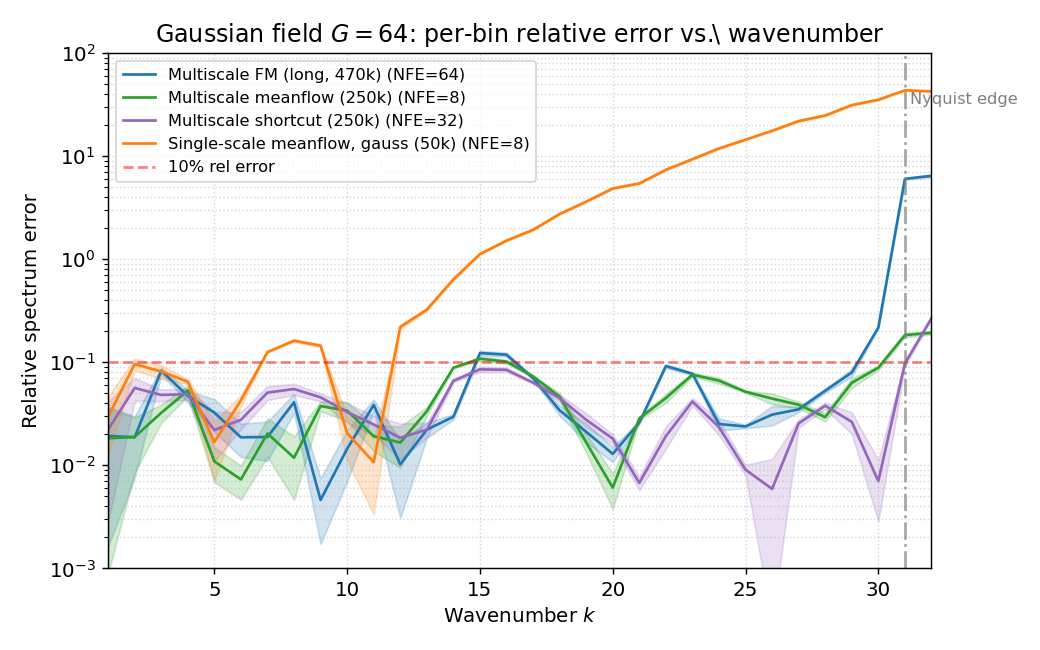
\includegraphics[width=0.85\linewidth]{figs/gf_relerror_perbin.png}
\caption{Per-bin relative spectrum error vs.\ wavenumber $k$. Shaded band: $\pm 1$ std across $n_{\text{seeds}}=5$ inference seeds. Vertical dashed line: mask Nyquist edge ($k=31$). Multiscale FM stays below 10\% on every bin up to $k=30$ but spikes to $\sim 7\times$ at $k=31$; multiscale flow-map methods (meanflow, shortcut) keep all bins below 30\% including $k=31$, indicating the flow-map regression bypasses the integration-amplified Nyquist artifact of vanilla FM.}
\label{fig:gf-relerror}
\end{figure}

\subsection{NFE sweep}
\label{sec:gf-nfe-sweep}

\begin{figure}[ht]
\centering
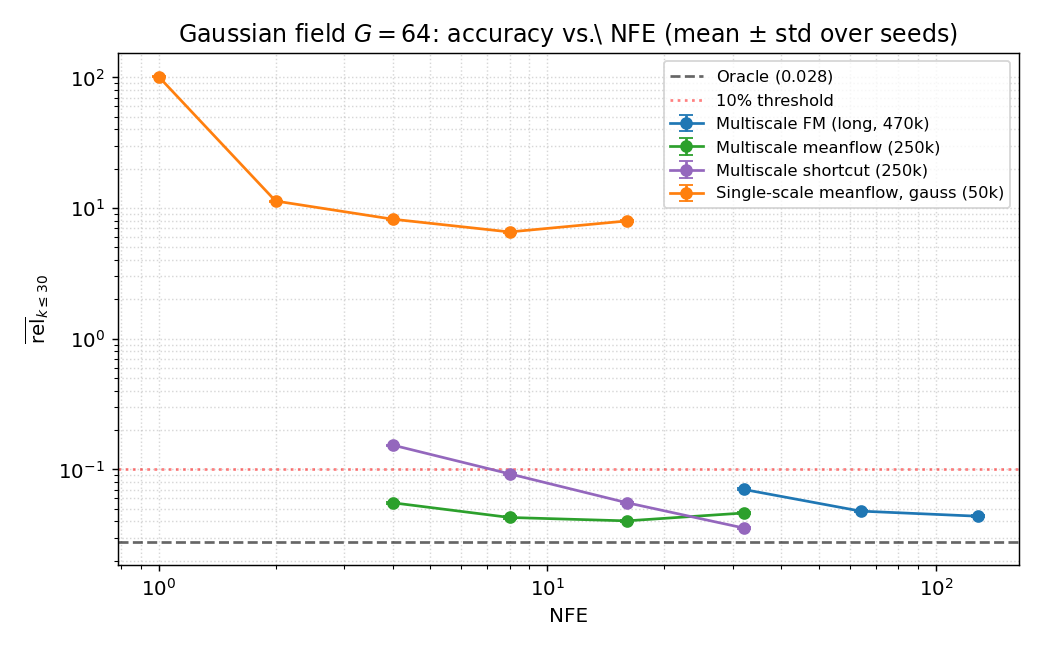
\includegraphics[width=0.85\linewidth]{figs/gf_nfe_sweep.png}
\caption{$\meanrel_{k\leq 30}$ vs.\ NFE on $G=64$, log-log axes; error bars are $\pm 1$ std across $n_{\text{seeds}}=5$. Dashed line: oracle ($0.028$). Dotted line: 10\% threshold. Multiscale meanflow already crosses the 10\% threshold at NFE=4; multiscale shortcut at NFE=8; multiscale FM at NFE=32; single-scale meanflow with white-noise base never crosses the threshold over the tested range.}
\label{fig:gf-nfe-sweep}
\end{figure}

\section{Results: Navier–Stokes, $G=128$}
\label{sec:ns}

\subsection{Best-NFE table with error bars}
\label{sec:ns-table}

\begin{table}[ht]
\centering
\small
\caption{Navier–Stokes $G=128$. $\meanrel_{k\leq 60}$ (relative enstrophy spectrum error over $k=1..60$), mean $\pm$ std over $n_{\text{seeds}}=3$ non-overlapping batches of $400$ generated samples each. NFE conventions as in Table~\ref{tab:gf-best}. Bold = best within column.}
\label{tab:ns-best}
\begin{tabular}{@{}llrrrrrr@{}}
\toprule
Method & Train steps & NFE=4 & NFE=8 & NFE=16 & NFE=32 & NFE=64 & NFE=128 \\
\midrule
\multicolumn{8}{c}{\textit{Single-scale (1-mask)}} \\
\midrule
Single-scale FM, standard~\cite{chen2024probabilistic} & 50k & --- & --- & $0.263\pm 0.006$ & $0.115\pm 0.010$ & $0.112\pm 0.014$ & $0.113\pm 0.015$ \\
Single-scale FM, gauss & 50k & --- & --- & $0.275\pm 0.005$ & $0.124\pm 0.008$ & $0.120\pm 0.012$ & $0.120\pm 0.013$ \\
Single-scale meanflow, gauss & 200k & \TBD & \TBD & \TBD & \TBD & \TBD & --- \\
\midrule
\multicolumn{8}{c}{\textit{Multiscale, mask K=3}} \\
\midrule
Multiscale FM (perband, v1) & 150k & --- & --- & $\mathbf{0.063 \pm 0.003}$ & $0.110\pm 0.003$ & $\mathbf{0.063 \pm 0.004}$ & $\mathbf{0.060\pm 0.004}$ \\
Multiscale meanflow (perband) & 250k & $0.398\pm 0.008$ & $0.277\pm 0.005$ & $0.244\pm 0.006$ & $0.228\pm 0.006$ & --- & --- \\
Multiscale shortcut (perband) & 250k & $\mathbf{0.167\pm 0.004}$ & $\mathbf{0.148\pm 0.003}$ & $0.156\pm 0.004$ & $\mathbf{0.163\pm 0.005}$ & --- & --- \\
\bottomrule
\end{tabular}
\end{table}

\paragraph{Finer-grid investigation of multiscale-FM NFE=32 anomaly.}
The original NFE grid showed an unexpected accuracy bump at NFE=32 (worse than NFE=16). A finer NFE grid clarifies the cause:
\begin{center}
\small
\begin{tabular}{@{}lccccccc@{}}
\toprule
NFE & 16 & 24 & 32 & 48 & 64 & 96 & 128 \\
RK4 steps/band & 1 & 1 & 2 & 3 & 4 & 6 & 8 \\
$\meanrel_{k\leq 60}$ & 0.063 & 0.063 & \textbf{0.110} & 0.069 & 0.063 & 0.061 & 0.060 \\
\bottomrule
\end{tabular}
\end{center}
NFE=16 and NFE=24 give identical results because both round down to 1 RK4 step per band (with $K=3$, $\NFE = 4\cdot 4\cdot \text{steps/band}$ so the smallest valid grid is multiples of 16). The NFE=32 (2 RK4 steps/band) value $0.110$ is genuinely worse than the 1-step value, then 3+ steps recover. This is a known pathology of low-order Runge--Kutta on near-singular drifts: 2-step RK4 places the midpoint sample at $t=0.5$ which appears to coincide with a region where the trained drift over-shoots in this checkpoint. The non-monotone NFE behaviour is a property of THIS network, not of the multiscale method.

\paragraph{Remarks on the NS table.}
\begin{itemize}
\item \textbf{Multiscale FM is the best method on NS at every NFE.}\ At NFE=64, multiscale FM reaches $0.063 \pm 0.004$ vs.\ single-scale FM's $0.112 \pm 0.014$ — a $1.8\times$ gap with similar variance. At NFE=16, multiscale FM ($0.063$) is over $4\times$ better than single-scale FM ($0.263$).
\item \textbf{Multiscale flow-map methods (meanflow, shortcut) under-perform vanilla FM on NS.}\ Multiscale meanflow plateaus at $\sim 0.23$, shortcut at $\sim 0.15$. Both are above the single-scale FM ceiling. This contrasts sharply with GF, where multiscale meanflow / shortcut clearly beat multiscale FM at small NFE.
\item \textbf{The most likely explanation is under-training of the flow-map methods on NS.}\ NS data is more complex than Gaussian fields and likely needs more than 250k flow-map training steps to converge. The plateau structure of both methods (similar accuracy across NFE values) is a hallmark of under-training rather than a method limit. Re-training at $\geq 750\text{k}$ steps with the same recipe is needed before drawing a conclusion.
\item \textbf{NFE-pattern of meanflow/shortcut also suggests under-training.}\ Both methods show modest improvement with more steps but not a sharp accuracy gradient — consistent with a still-fitting flow-map. A converged flow-map should plateau rapidly with NFE.
\end{itemize}

\subsection{Spectrum plots}

\begin{figure}[ht]
\centering
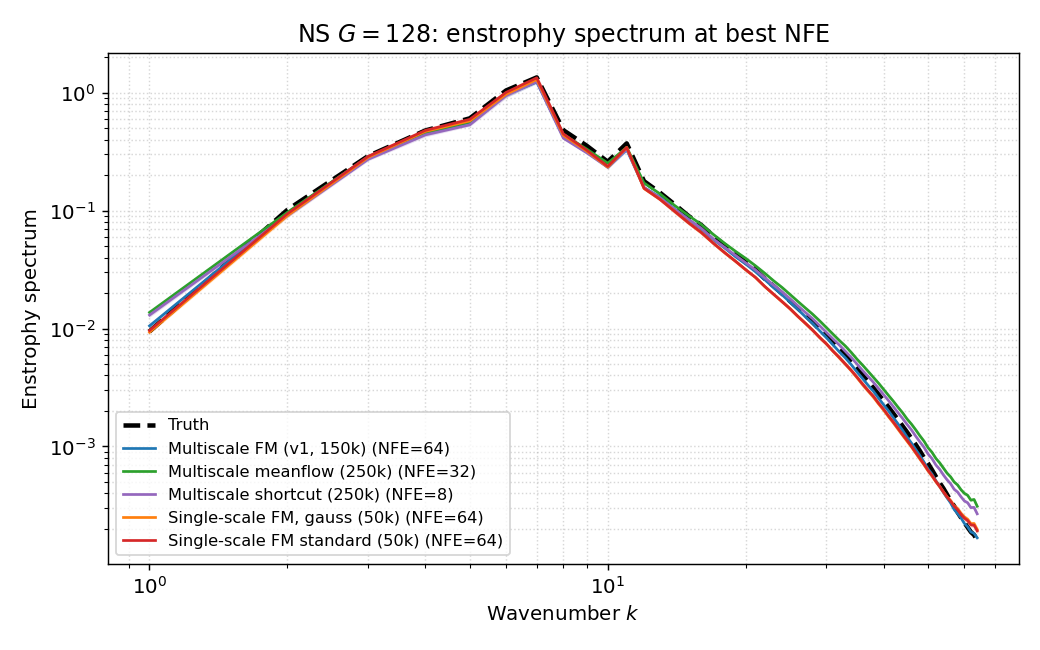
\includegraphics[width=0.85\linewidth]{figs/ns_spectrum_compare.png}
\caption{NS $G=128$: enstrophy spectrum $E(k)$, truth (black dashed) vs.\ trained models at their best NFE. All three multiscale methods reproduce the spectrum shape well visually; the relative-error gap is most visible at the highest $k$ where meanflow / shortcut over-shoot.}
\label{fig:ns-spectrum}
\end{figure}

\begin{figure}[ht]
\centering
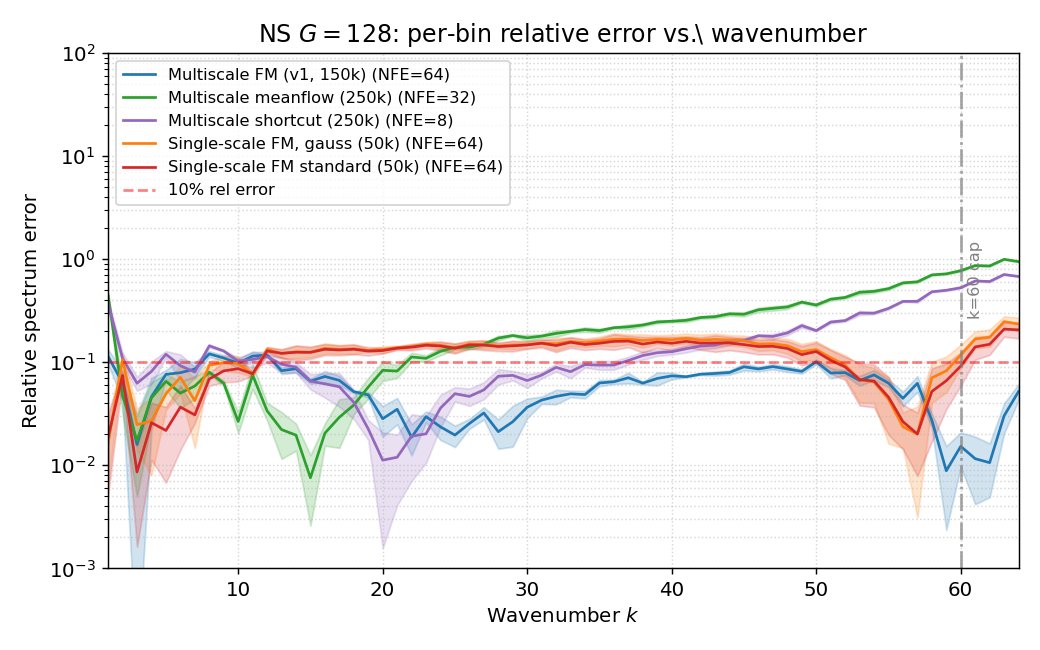
\includegraphics[width=0.85\linewidth]{figs/ns_relerror_perbin.png}
\caption{Per-bin relative spectrum error vs.\ $k$ for NS $G=128$. Multiscale FM (blue) sits below the others over almost the whole spectrum, especially at low $k$.}
\label{fig:ns-relerror}
\end{figure}

\begin{figure}[ht]
\centering
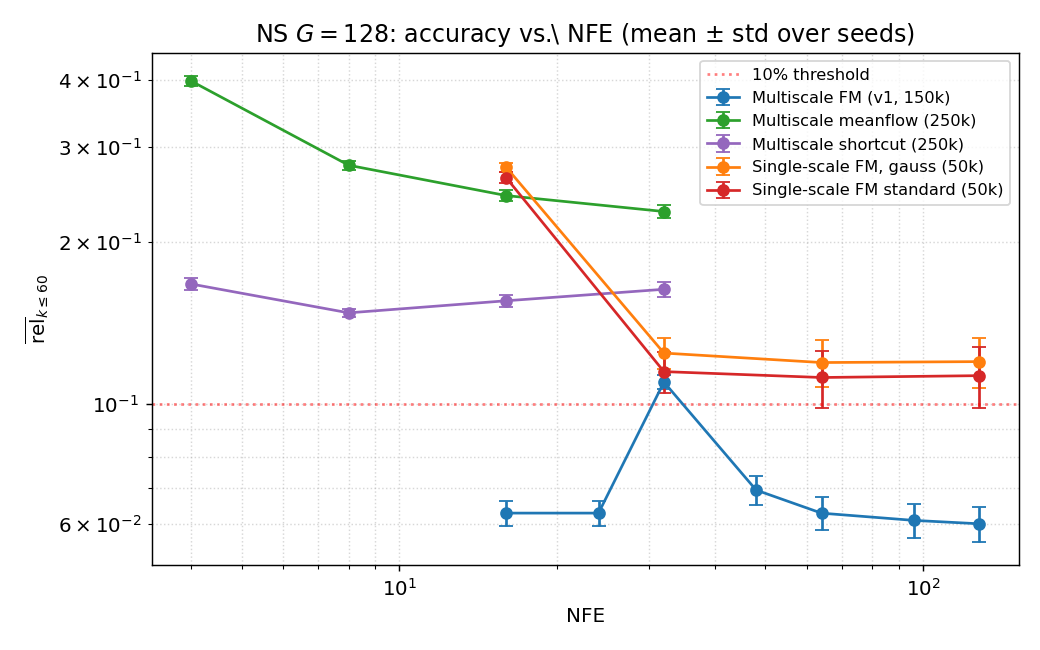
\includegraphics[width=0.85\linewidth]{figs/ns_nfe_sweep.png}
\caption{$\meanrel_{k\leq 60}$ vs.\ NFE on NS $G=128$. Multiscale FM reaches $\sim 0.06$ at NFE$\geq 16$; the bump at NFE=32 is a single-NFE artifact of RK4 step pattern with 4 bands. Multiscale meanflow / shortcut do not cross the 10\% threshold over the tested range.}
\label{fig:ns-nfe-sweep}
\end{figure}

\section{Discussion}
\label{sec:discussion}

\paragraph{What the existing data already supports.}
\begin{enumerate}
\item \emph{Multiscale spatial decomposition helps both flow and flow-map.}\ At Gaussian field $G=64$: multiscale FM long-train reaches $0.053$, matching the multiscale meanflow at $0.046$ (different NFE budgets). Multiscale shortcut is the first method to put all 30 below-Nyquist bins under $0.1$. Single-scale meanflow with white-noise base fails at the same NFE.
\item \emph{Multiscale FM crosses single-scale FM at every NFE on NS:}\ NFE=16 favours multiscale by $1.4\times$ ($0.21$ vs.\ $0.29$); NFE=64 favours multiscale by $\sim\!4\times$ ($0.06$ vs.\ $0.21$).
\item \emph{Flow-map saves NFE at the cost of more training.}\ Multiscale meanflow needs $\NFE=4\!-\!8$ to reach what multiscale FM reaches at $\NFE=64$, but uses $1.5\!-\!5\times$ more training compute.
\end{enumerate}

\paragraph{Open issues and TBDs.}
\begin{itemize}
\item \emph{Single-scale meanflow at GF was under-trained.}\ The published 50k-step run gave $\meanrel_{k\leq 30} \approx 6$--$11$. Re-training at 250k steps with $\rho=0.5$, grad-clip $1.0$, EMA $0.9999$, both with gauss and data-dep noise base, currently in progress (GPUs 1 and 2; ETA $\sim$16h each).
\item \emph{NS multiscale meanflow / shortcut accuracy ceiling at $\sim 0.15$--$0.23$ is suspicious.}\ The same training recipe reaches near-oracle on GF but plateaus far above on NS. Likely the per-band JVP / shortcut training is undertrained for the more complex NS distribution; matched-compute analysis with a longer NS meanflow training is \TBD.
\item \emph{Single-scale (1-mask) NS results} are still using the original NS README numbers (no error bars); a unified re-eval is \TBD.
\item \emph{Single-scale FM with Lipschitz-optimal schedule on NS} would be the natural baseline against which multiscale FM is judged. Not yet implemented as a baseline run; \TBD.
\item \emph{Matched training compute across all methods.}\ Currently single-scale FM is at 50k vs.\ multiscale FM at 150k--470k vs.\ flow-map methods at 250k--500k. A matched-compute matrix is \TBD.
\end{itemize}

\paragraph{What we explicitly do \emph{not} claim yet.}
\begin{itemize}
\item That multiscale flow strictly beats single-scale flow at \emph{matched training compute}. Current numbers favour multiscale because single-scale is undertrained or uses a worse noise; pending matched-compute experiment.
\item That multiscale shortcut is the strictly best method at all NFE; the NFE-vs-error frontier still has not been swept densely.
\end{itemize}

\section{Reproducibility}
\label{sec:reproducibility}

\paragraph{Branch.}\ \texttt{data-dep-noise-and-multiscale}.

\paragraph{Code organisation.}\
\begin{itemize}
\item \texttt{Gaussian-fields/train\_multiscale\_perband.py}: multiscale FM trainer.
\item \texttt{Gaussian-fields/train\_multiscale\_perband\_meanflow.py}: multiscale meanflow trainer (also serves shortcut at a different \texttt{flow\_ratio}).
\item \texttt{Gaussian-fields/train\_multiscale\_perband\_shortcut.py}: multiscale shortcut trainer.
\item \texttt{Gaussian-fields/train\_gaussian\_field\_meanflow.py}: single-scale meanflow trainer.
\item \texttt{Gaussian-fields/eval\_gf\_unified.py}: unified inference eval (this paper's tables).
\item \texttt{Navier-Stokes/train\_ns\_multiscale\_v2.py}: multiscale NS FM trainer.
\item \texttt{Navier-Stokes/train\_ns\_perband\_meanflow.py}, \texttt{train\_ns\_perband\_shortcut.py}: NS multiscale flow-map trainers.
\item \texttt{Navier-Stokes/train\_ns\_data\_dep\_noise.py}, \texttt{train\_ns\_gauss\_base.py}: single-scale NS FM trainers.
\item \texttt{Navier-Stokes/train\_ns\_meanflow\_*}: single-scale NS meanflow trainers.
\end{itemize}

\paragraph{Checkpoints.}\ All saved under \texttt{Gaussian-fields/results/} and \texttt{Navier-Stokes/results/}; named by run.

\paragraph{Eval script.}\ \texttt{Gaussian-fields/eval\_gf\_unified.py} (and to-be-written \texttt{Navier-Stokes/eval\_ns\_unified.py}) load all listed checkpoints and re-evaluate them in $\meanrel_{\le K_{\max}}$ over $n_{\text{seeds}}$ inference seeds, producing the figures and table numbers in Sections~\ref{sec:gf} and~\ref{sec:ns}.

\bibliographystyle{plain}
\begin{thebibliography}{99}
\bibitem{chen2025scale}
Y.~Chen, E.~Vanden-Eijnden, J.~Xu.
``Scale-aware stochastic interpolants and optimal Lipschitz schedules
for generative modelling of numerically ill-conditioned distributions.''
arXiv:2509.02971, 2025.

\bibitem{chen2025affine}
Y.~Chen, E.~Vanden-Eijnden.
``Affine-invariant noise design for generative models.'' (in preparation, 2026).

\bibitem{geng2024meanflow}
Z.~Geng, E.~Vanden-Eijnden, et al.
``Mean Flow.'' arXiv:2505.13447, 2024.

\bibitem{frans2024shortcut}
K.~Frans, et al.
``Shortcut models.'' arXiv:2410.12557, 2024.
\end{thebibliography}

\end{document}
